\documentclass[11pt,a4paper]{article}
\usepackage{amsmath}
\usepackage{amsfonts}
\usepackage{amssymb}
\usepackage{makeidx}
\usepackage{graphicx}
\usepackage{wrapfig}
\usepackage{enumerate}
\usepackage{pdfpages}
\usepackage{tocloft}
\usepackage{setspace}
\usepackage{mathtools}
\usepackage{hyperref}
\definecolor{linkcolour}{rgb}{0,0.2,0.6} % Link color
\hypersetup{colorlinks,breaklinks,urlcolor=linkcolour,linkcolor=linkcolour}

\usepackage[left=2cm,right=2cm,top=1.5cm,bottom=1.5cm]{geometry}

\usepackage{xcolor}

\usepackage{color,soul}
\usepackage{fontspec}
\setmainfont{Cambria}

\usepackage{caption}
\captionsetup[figure]{font=small, labelfont={bf}}
\captionsetup[table]{font=small, labelfont={bf}}

\usepackage{float}
\usepackage{multirow}
\usepackage{longtable}

\usepackage[nottoc]{tocbibind}

\newcommand{\spa}{\vspace{1.25em}}
\newcommand{\noi}{\noindent}
\def\dul#1{\underline{\underline{#1}}}
\def\cpt#1#2{{\begin{center}\small\textbf{\textcolor{blue}{Figure #1:}} #2\end{center}}}
\def\tt#1{\texttt{#1}}
\def\colortt#1{\textcolor{blue}{\texttt{#1}}}

% for dots in the content
\usepackage{tocloft}
\renewcommand{\cftsecleader}{\cftdotfill{\cftdotsep}}

% For getting paragraphs
\usepackage{titlesec}
\setcounter{secnumdepth}{4}
\setcounter{tocdepth}{4}
\titleformat{\paragraph}
{\normalfont\normalsize\bfseries}{\theparagraph}{1em}{}
\titlespacing*{\paragraph}
{0pt}{3.25ex plus 1ex minus .2ex}{1.5ex plus .2ex}

\begin{document}
	\begin{titlepage} 
		\begin{center}
		\large{ASSIGNMENT 3}\\
		\vspace{2em}
		\large {CS5691 Pattern Recognition and Machine Learning}
		\vspace{3em}
		
		\rule{0.9\linewidth}{0.5mm} \\[0.4cm]
	    {\Large{\bfseries{CS5691 Assignment 3}}} \\
	    \rule{0.9\linewidth}{0.5mm} \\[3 em]	
	    
	    Team Members: \\
	    \vspace{0.5em}
	   	\def\arraystretch{1.25}
\begin{tabular}{c l}
	\hline
	BE17B007 & N Sowmya Manojna \\
	PH17B010 & Thakkar Riya Anandbhai \\
	PH17B011 & Chaithanya Krishna Moorthy \\
	\hline
\end{tabular}

		\vspace{1em}

		Indian Institute of Technology, Madras\\    
		
		\vspace{5em}    
	    
	    	
\includegraphics[scale=0.09]{images/iitmlogo.png}
		\end{center}
	\end{titlepage}

{\hypersetup{linkcolor=black}
 \tableofcontents}
\break


%%%%%%%%%%%%%%%%%%%%%%%%%%%%%%%%%%%%%%%%%%%%%%%
%%%%%%%%%%%%%%%%%%%%%%%%%%%%%%%%%%%%%%%%%%%%%%%
\section{Dataset 1A}
This dataset contains data for four classes - 0, 1, 2 and 3. The classes are linearly separable and the dimension of the feature space is 2.
%%%%%%%%%%%%%%%%%%%%%%%%%%%%%%%%%%%%%%%%%%%%%%%
%%%%%%%%%%%%%%%%%%%%%%%%%%%%%%%%%%%%%%%%%%%%%%%
\subsection{Perceptron}
%%%%%%%%%%%%%%%%%%%%%%%%%%%%%%%%%%%%%%%%%%%%%%%%%%
Varying the hyperparameter : Learning Rate ($\eta$) for the Perceptron model, the accuracies on the training and validation (30\% of the file \colortt{dev.csv}) data for all possible pairings of the classes (leading to a total of 6 pairs ) were obtained and the best $\eta$ value based on CV accuracies was chosen as follows:

%%%%%%%%%%%%%%%%%%%%%%%%%%%%%%%%%%%%%%%%%%%%%%%%%%
\subsubsection{Classes 0 and 1}
%%%%%%%%%%%%%%%%%%%%%%%%%%%%%%%%%%%%%%%%%%%%%%%%%%
\def\arraystretch{1.25}
\begin{center}
{\small
\begin{tabular}{l l l c}
\hline
\hline
\textbf{Hyperparameter}&\textbf{Training Accuracy} & \textbf{CV Accuracy}\\
\hline
\hline
0.001&1.0&1.0\\
0.005&1.0&1.0\\
0.01&1.0&1.0\\
0.05&1.0&1.0\\
0.1&1.0&1.0\\
1.0&1.0&1.0\\
5.0&1.0&1.0\\
10.0&1.0&1.0\\
100.0&1.0&1.0\\
\hline
\end{tabular}

\captionof{table}{Table of training accuracies and CV accuracies for data of classes 0 and 1 of the 1A data set}
}
\end{center}

\noi
The accuracy is 100\% for all values of the hyperparameters. Taking the default value of 0.01, the accuracy on the test data is \textbf{100\%}. The confusion matrices for the training and test data are as in \autoref{fig:perc_conf_01}.
\begin{figure}[H]
    \centering
    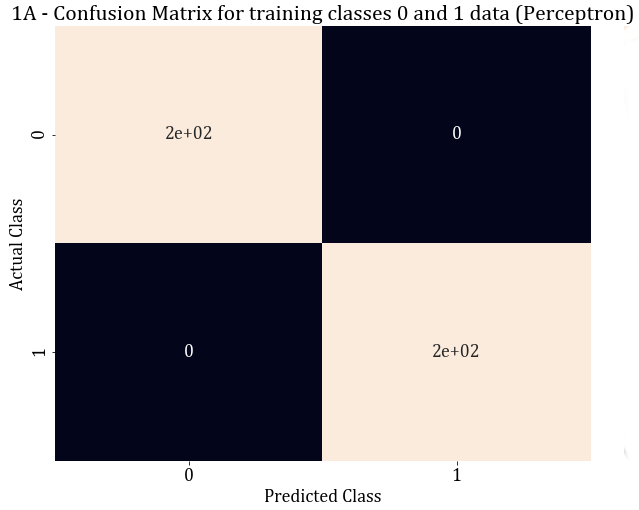
\includegraphics[scale=0.35]{images/1A_perceptron_training_classes_0_and_1_confmat.png}
    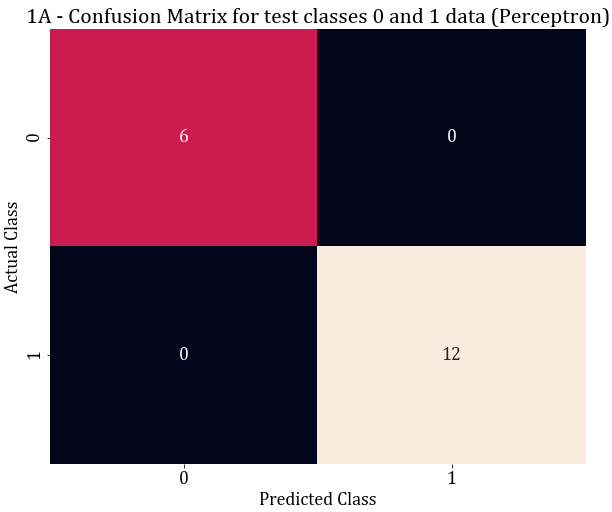
\includegraphics[scale=0.35]{images/1A_perceptron_test_classes_0_and_1_confmat.png}
    \caption{Confusion matrices for training and test data belonging to classes 0 and 1 of data 1A using perceptron classifier}
    \label{fig:perc_conf_01}
\end{figure}

\noi
The decision region plot for the perceptron classifier is in \autoref{fig:perc_dec_reg_01}.
\begin{figure}[H]
    \centering
    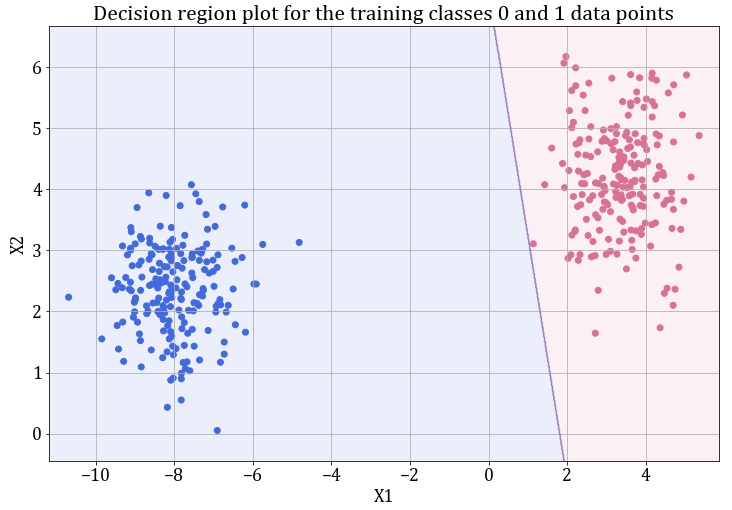
\includegraphics[scale=0.45]{images/1A_perceptron_training_classes_0_and_1_dec_reg.png}
    \caption{Decision region plot for classes 0 and 1 of data 1A using perceptron classifier}
    \label{fig:perc_dec_reg_01}
\end{figure}

%%%%%%%%%%%%%%%%%%%%%%%%%%%%%%%%%%%%%%%%%%%%%%%%%%
\subsubsection{Classes 0 and 2}
%%%%%%%%%%%%%%%%%%%%%%%%%%%%%%%%%%%%%%%%%%%%%%%%%%
\def\arraystretch{1.25}
\begin{table}[H]
{\small
\centering
\begin{tabular}{l l l c}
\hline
\hline
\textbf{Hyperparameter} & \textbf{Training Accuracy}  &  \textbf{CV Accuracy}\\
\hline
\hline
0.001 & 100.0 & 100.0\\
0.005 & 100.0 & 100.0\\
0.01 & 100.0 & 100.0\\
0.05 & 100.0 & 100.0\\
0.1 & 100.0 & 100.0\\
1.0 & 100.0 & 100.0\\
5.0 & 100.0 & 100.0\\
10.0 & 100.0 & 100.0\\
100.0 & 100.0 & 100.0\\
\hline
\end{tabular}
\caption{Training and CV accuracies for classes 0 and 2 of dataset 1A.}
}
\end{table}

\noi
The accuracy is 100\% for all values of the hyperparameters. Taking the default value of 0.01, the accuracy on the test data is \textbf{100\%}. The confusion matrices for the training and test data are as in \autoref{fig:perc_conf_02}.
\begin{figure}[H]
    \centering
    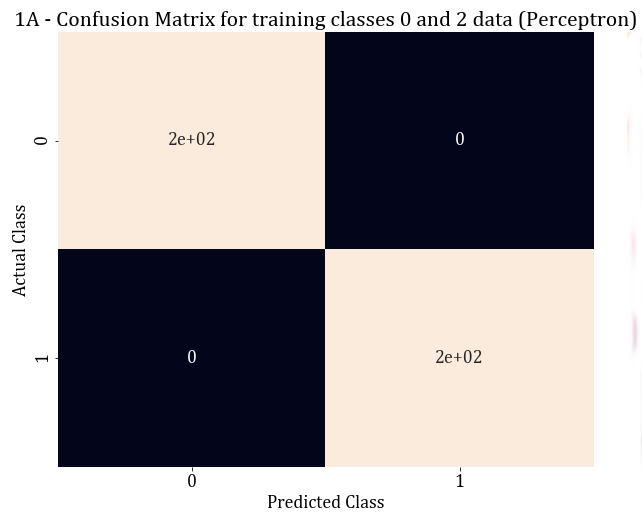
\includegraphics[scale=0.35]{images/1A_perceptron_training_classes_0_and_2_confmat.png}
    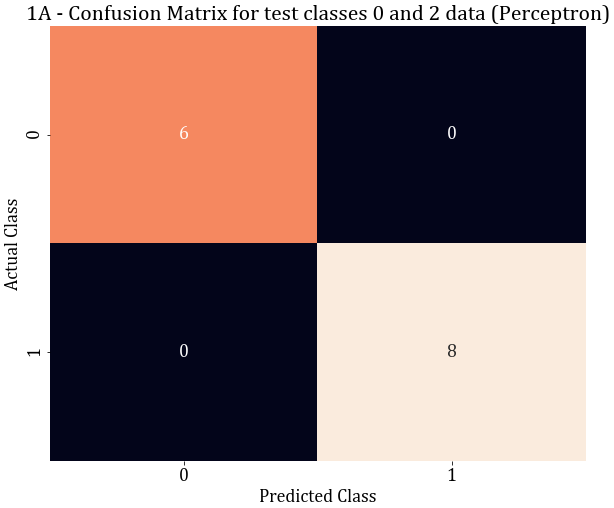
\includegraphics[scale=0.35]{images/1A_perceptron_test_classes_0_and_2_confmat.png}
    \caption{Confusion matrices for training and test data belonging to classes 0 and 2 of data 1A using perceptron classifier}
    \label{fig:perc_conf_02}
\end{figure}

\noi
The decision region plot for the perceptron classifier is in \autoref{fig:perc_dec_reg_02}.
\begin{figure}[H]
    \centering
    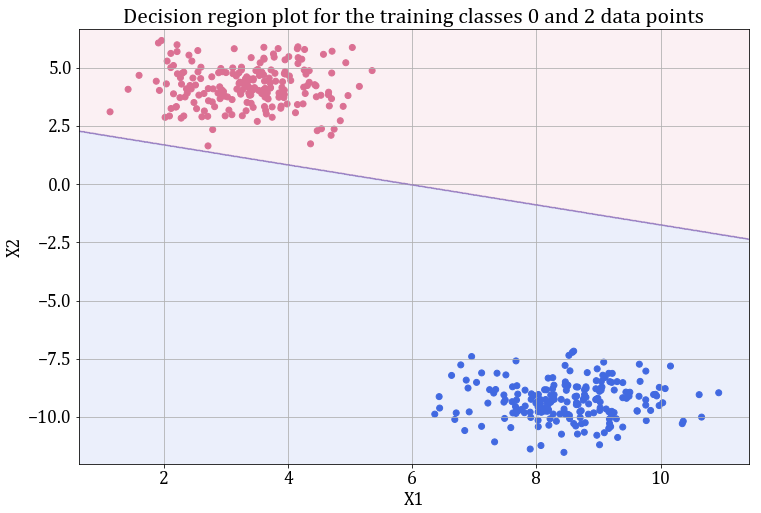
\includegraphics[scale=0.45]{images/1A_perceptron_training_classes_0_and_2_dec_reg.png}
    \caption{Decision region plot for classes 0 and 2 of data 1A using perceptron classifier}
    \label{fig:perc_dec_reg_02}
\end{figure}

%%%%%%%%%%%%%%%%%%%%%%%%%%%%%%%%%%%%%%%%%%%%%%%%%%
\subsubsection{Classes 0 and 3}
%%%%%%%%%%%%%%%%%%%%%%%%%%%%%%%%%%%%%%%%%%%%%%%%%%
\def\arraystretch{1.25}
\begin{center}
{\small
\begin{tabular}{l l l c}
\hline
\hline
\textbf{Hyperparameter}&\textbf{Training Accuracy} & \textbf{CV Accuracy}\\
\hline
\hline
0.001&1.0&1.0\\
0.005&1.0&1.0\\
0.01&1.0&1.0\\
0.05&1.0&1.0\\
0.1&1.0&1.0\\
1.0&1.0&1.0\\
5.0&1.0&1.0\\
10.0&1.0&1.0\\
100.0&1.0&1.0\\
\hline

\end{tabular}

\captionof{table}{Table of training accuracies and CV accuracies for data of classes 0 and 3 of the 1A data set}
}
\end{center}

The accuracy is 100\% for all values of the hyperparameters. Taking the default value of 0.01, the accuracy on the test data is \textbf{100\%}. The confusion matrices for the training and test data are as in \autoref{fig:perc_conf_03}.
\begin{figure}[H]
    \centering
    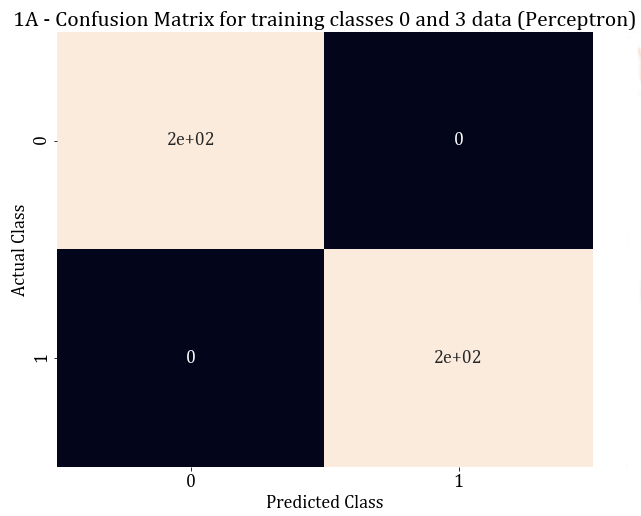
\includegraphics[scale=0.3]{images/1A_perceptron_training_classes_0_and_3_confmat.png}
    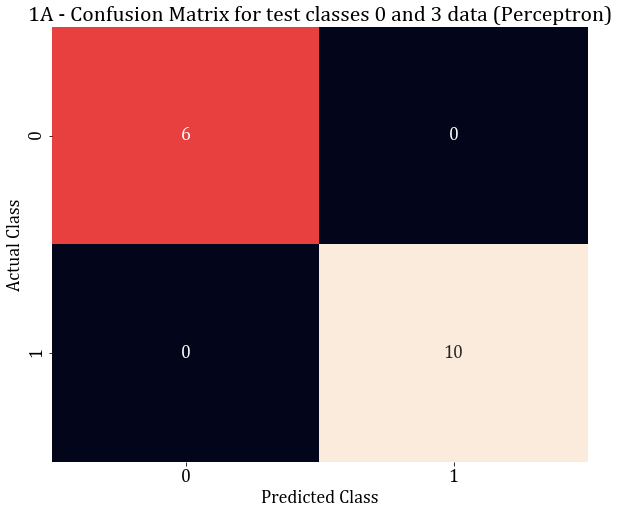
\includegraphics[scale=0.3]{images/1A_perceptron_test_classes_0_and_3_confmat.png}
    \caption{Confusion matrices for training and test data belonging to classes 0 and 3 of data 1A using perceptron classifier}
    \label{fig:perc_conf_03}
\end{figure}
The decision region plot for the perceptron classifier is in \autoref{fig:perc_dec_reg_03}.
\begin{figure}[H]
    \centering
    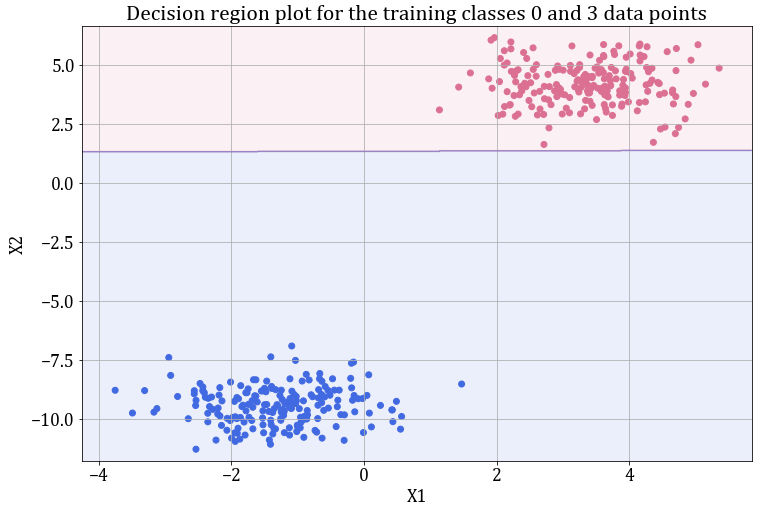
\includegraphics[scale=0.45]{images/1A_perceptron_training_classes_0_and_3_dec_reg.png}
    \caption{Decision region plot for classes 0 and 3 of data 1A using perceptron classifier}
    \label{fig:perc_dec_reg_03}
\end{figure}

%%%%%%%%%%%%%%%%%%%%%%%%%%%%%%%%%%%%%%%%%%%%%%%%%%
\subsubsection{Classes 1 and 2}
%%%%%%%%%%%%%%%%%%%%%%%%%%%%%%%%%%%%%%%%%%%%%%%%%%
\def\arraystretch{1.25}
\begin{center}
{\small
\begin{tabular}{l l l c}
\hline
\hline
\textbf{Hyperparameter}&\textbf{Training Accuracy} & \textbf{CV Accuracy}\\
\hline
\hline
0.001&1.0&0.975\\
0.005&1.0&0.975\\
0.01&1.0&0.975\\
0.05&1.0&1.0\\
0.1&1.0&1.0\\
1.0&1.0&1.0\\
5.0&1.0&1.0\\
10.0&1.0&1.0\\
100.0&1.0&1.0\\
\hline
\end{tabular}

\captionof{table}{Table of training accuracies and CV accuracies for data of classes 1 and 2 of the 1A data set}
}
\end{center}

The accuracy on the CV data is best for $\eta = 0.05$. Using this value for the perceptron model, the accuracy on the test data is \textbf{100\%}. The confusion matrices for the training and test data are as in \autoref{fig:perc_conf_12}.

\begin{figure}[H]
    \centering
    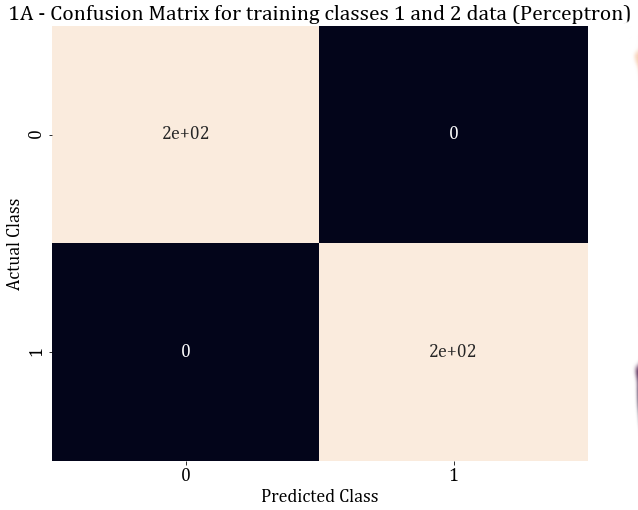
\includegraphics[scale=0.3]{images/1A_perceptron_training_classes_1_and_2_confmat.png}
    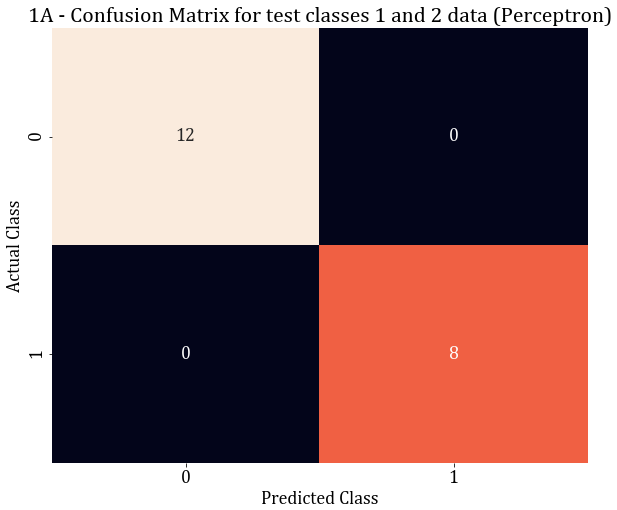
\includegraphics[scale=0.3]{images/1A_perceptron_test_classes_1_and_2_confmat.png}
    \caption{Confusion matrices for training and test data belonging to classes 1 and 2 of data 1A using perceptron classifier}
    \label{fig:perc_conf_12}
\end{figure}
The decision region plot for the perceptron classifier is in \autoref{fig:perc_dec_reg_12}.
\begin{figure}[H]
    \centering
    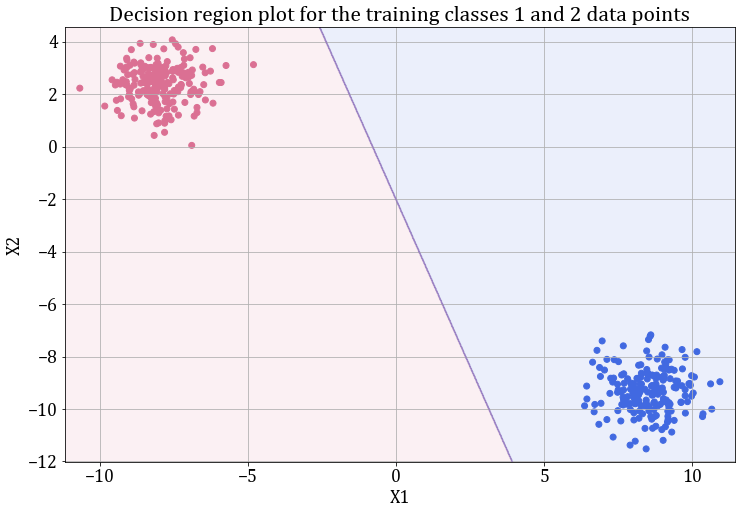
\includegraphics[scale=0.45]{images/1A_perceptron_training_classes_1_and_2_dec_reg.png}
    \caption{Decision region plot for classes 1 and 2 of data 1A using perceptron classifier}
    \label{fig:perc_dec_reg_12}
\end{figure}

%%%%%%%%%%%%%%%%%%%%%%%%%%%%%%%%%%%%%%%%%%%%%%%
\subsubsection{Classes 1 and 3}
%%%%%%%%%%%%%%%%%%%%%%%%%%%%%%%%%%%%%%%%%%%%%%%%%%
\def\arraystretch{1.25}
\begin{table}[H]
{\small
\centering
\begin{tabular}{l l l l l l}
\hline
\hline
\textbf{Hyperparameter}&\textbf{Training Accuracy} & \textbf{CV Accuracy} & \textbf{Hyperparameter}&\textbf{Training Accuracy} & \textbf{CV Accuracy}\\
\hline
\hline
0.001 & 100.0 & 100.0 & 1.0 & 100.0 & 100.0\\
0.005 & 100.0 & 100.0 & 5.0 & 100.0 & 100.0\\
0.01 & 100.0 & 100.0 & 10.0 & 100.0 & 100.0\\
0.05 & 100.0 & 100.0 & 100.0 & 100.0 & 100.0\\
0.1 & 100.0 &100.0 & & & \\
\hline
\end{tabular}
\caption{Training and CV accuracies for classes 1 and 3 of dataset 1A.}
}
\end{table}
The accuracy is 100\% for all values of the hyperparameters. Taking the default value of 0.01, the accuracy on the test data is \textbf{100\%}. The confusion matrices for the training and test data are as in \autoref{fig:perc_conf_13}.
\begin{figure}[H]
    \centering
    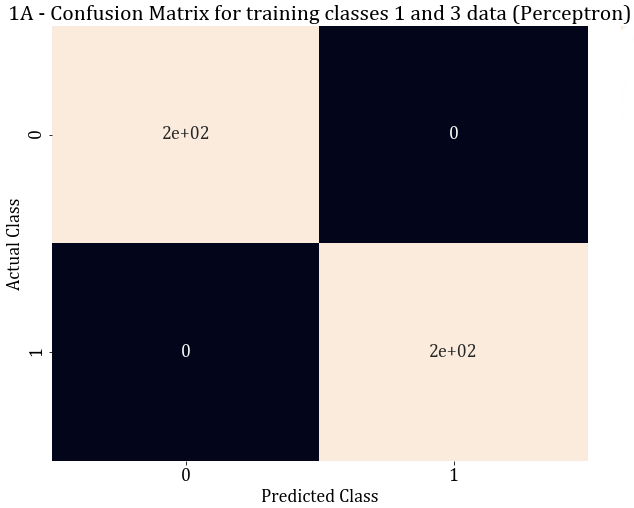
\includegraphics[scale=0.3]{images/1A_perceptron_training_classes_1_and_3_confmat.png}
    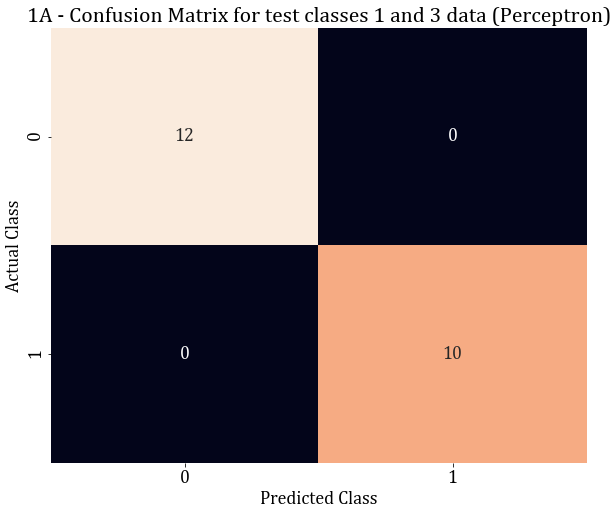
\includegraphics[scale=0.3]{images/1A_perceptron_test_classes_1_and_3_confmat.png}
    \caption{Confusion matrices for training and test data belonging to classes 1 and 3 of data 1A using perceptron classifier}
    \label{fig:perc_conf_13}
\end{figure}

\noi
The decision region plot for the perceptron classifier is in \autoref{fig:perc_dec_reg_13}.
\begin{figure}[H]
    \centering
    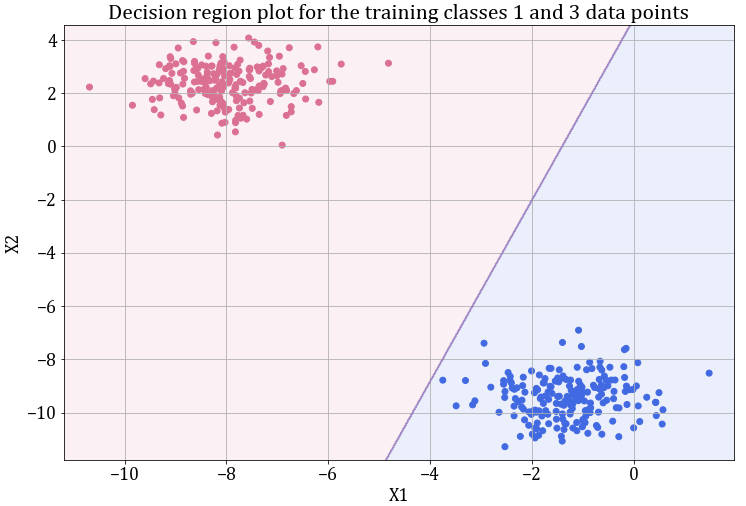
\includegraphics[scale = 0.45]{images/1A_perceptron_training_classes_1_and_3_dec_reg.png}
    \caption{Decision region plot for classes 1 and 3 of data 1A using perceptron classifier}
    \label{fig:perc_dec_reg_13}
\end{figure}


%%%%%%%%%%%%%%%%%%%%%%%%%%%%%%%%%%%%%%%%%%%%%%%
\subsubsection{Classes 2 and 3}
%%%%%%%%%%%%%%%%%%%%%%%%%%%%%%%%%%%%%%%%%%%%%%%%%%
\def\arraystretch{1.25}
\begin{table}[H]
{\small
\centering
\begin{tabular}{l l l l l l}
\hline
\hline
\textbf{Hyperparameter}&\textbf{Training Accuracy} & \textbf{CV Accuracy} & \textbf{Hyperparameter}&\textbf{Training Accuracy} & \textbf{CV Accuracy}\\
\hline
\hline
0.001 & 100.0 & 92.86 & 1.0 & 100.0 & 100.0\\
0.005 & 100.0 & 100.0 & 5.0 & 100.0 & 97.62\\
0.01 & 100.0 & 100.0 & 10.0 & 100.0 & 100.0\\
0.05 & 100.0 & 100.0 & 100.0 & 100.0 & 100.0\\
0.1 & 100.0 & 100.0 & & & \\
\hline
\end{tabular}
\caption{Training and CV accuracies for classes 2 and 3 of dataset 1A.}
}
\end{table}
The accuracy on the CV data is best for $\eta$ greater than or equal to 0.005. Using the default value of $\eta = 0.01$ for the perceptron model, the accuracy on the test data is \textbf{100\%}. The confusion matrices for the training and test data are as in \autoref{fig:perc_conf_23}.
\begin{figure}[H]
    \centering
    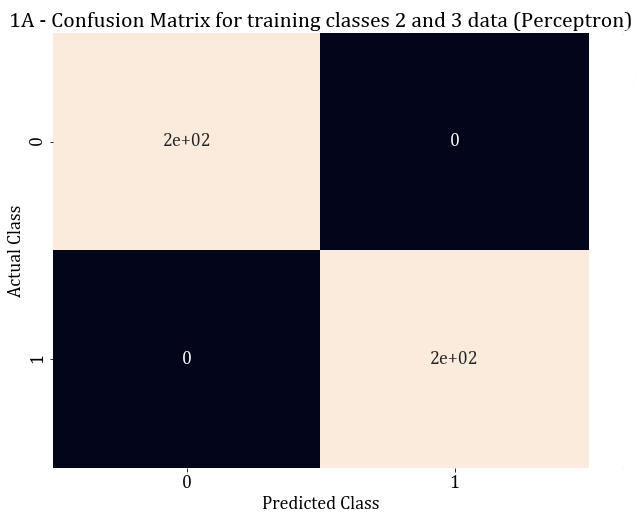
\includegraphics[scale=0.35]{images/1A_perceptron_training_classes_2_and_3_confmat.png}
    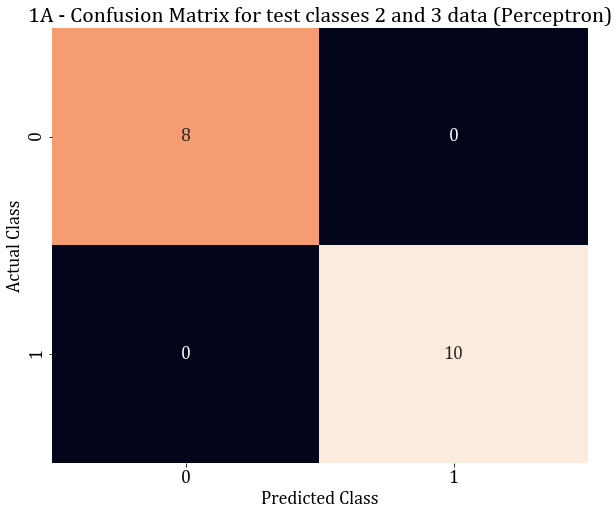
\includegraphics[scale=0.35]{images/1A_perceptron_test_classes_2_and_3_confmat.png}
    \caption{Confusion matrices for training and test data belonging to classes 2 and 3 of data 1A using perceptron classifier}
    \label{fig:perc_conf_23}
\end{figure}

\noi
The decision region plot for the perceptron classifier is in \autoref{fig:perc_dec_reg_23}.
\begin{figure}[H]
    \centering
    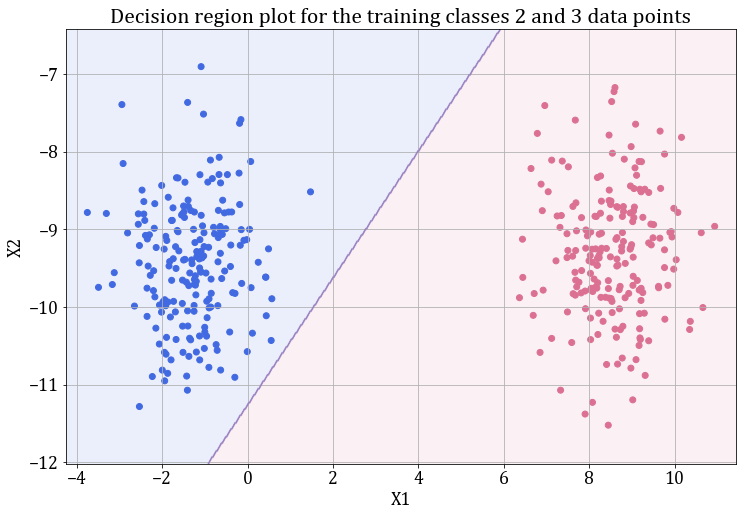
\includegraphics[scale = 0.45]{images/1A_perceptron_training_classes_2_and_3_dec_reg.png}
    \caption{Decision region plot for classes 2 and 3 of data 1A using perceptron classifier}
    \label{fig:perc_dec_reg_23}
\end{figure}

%%%%%%%%%%%%%%%%%%%%%%%%%%%%%%%%%%%%%%%%%%%%%%%
\subsection{MLFFNN}
%%%%%%%%%%%%%%%%%%%%%%%%%%%%%%%%%%%%%%%%%%%%%%%%%%
The hyperparameters varied and sweeped for are - \tt{hidden layer size}, \tt{optimizer}, \tt{batch size}, \tt{learning rate}, \tt{L2 regularization $\alpha$}.

\subsubsection{Classification Accuracies}
The classification accuracies on the training and validation datasets (30\% of the \colortt{dev.csv}) are as follows:
\def\arraystretch{1.25}
\begin{center}
{\small
\begin{tabular}{l l l l l l l c}
\hline
\hline
\textbf{\# Neurons} & \textbf{Activation} & \textbf{Solver} & \textbf{Batch Size} & \textbf{\alpha} & \textbf{Learning Rate} & \textbf{Accuracy} & \textbf{Validation Accuracy} \\
\hline
\hline
5 & tanh & lbfgs & 200 & 0.0001 & adaptive & 100.0 & 100.0 \\
5 & tanh & lbfgs & 200 & 0.0001 & constant & 100.0 & 100.0 \\
5 & tanh & lbfgs & 200 & 0.0 & invscaling & 100.0 & 100.0 \\
5 & tanh & lbfgs & 200 & 0.0 & adaptive & 100.0 & 100.0 \\
5 & tanh & lbfgs & 200 & 0.0 & constant & 100.0 & 100.0 \\
5 & tanh & lbfgs & 100 & 0.0 & adaptive & 100.0 & 100.0 \\
5 & tanh & lbfgs & 100 & 0.0001 & invscaling & 100.0 & 100.0 \\
5 & relu & lbfgs & 200 & 0.0 & constant & 100.0 & 100.0 \\
5 & relu & lbfgs & 100 & 0.0001 & invscaling & 100.0 & 100.0 \\
5 & relu & lbfgs & 200 & 0.0 & adaptive & 100.0 & 100.0 \\
\hline
\end{tabular}
\setcounter{table}{1}
\captionof{table}{Best 10 Train and Validation Accuracies obtained after performing a \colortt{GridSearch} on 432 parameter combinations.}
}
\end{center}

\subsubsection{Best Model}
The parameter combination were additionally sorted based on minimum fitting time (least fitting time - first) and the model that gave the best accuracy the fastest (and potentially the most minimal model that best fits the data), was chosen. Hence the best parameter combination chosen is:
\begin{itemize}
    \itemsep0em
    \item hidden\_layer\_sizes: 5
    \item activation: tanh
    \item solver: lbfgs
    \item batch\_size: 200
    \item alpha: 0.0001
    \item learning\_rate: adaptive
\end{itemize}

\noi
The classification accuracy of the best model on the testing data is: $100\%$. The confusion matrices obtained are as follows:
\begin{figure}[H]
    \centering
    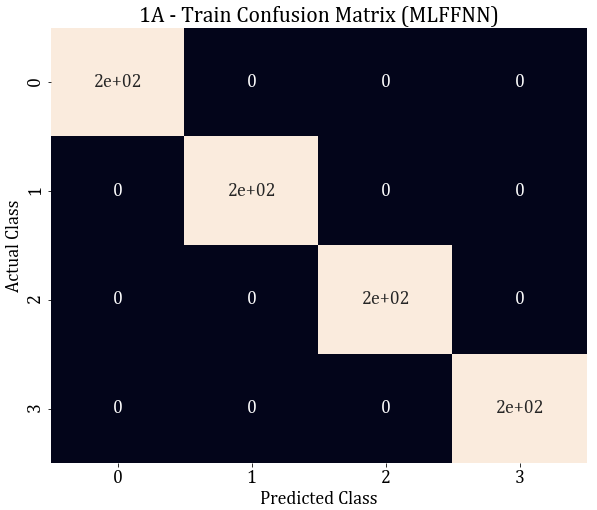
\includegraphics[scale=0.4]{images/1A_MLFFNN_train_confmat.png}
    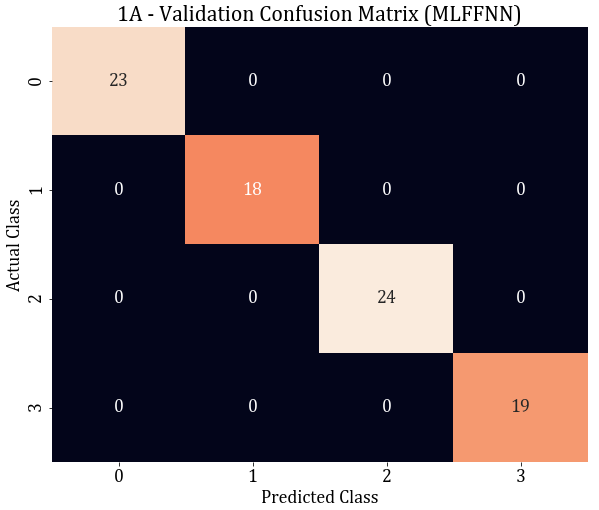
\includegraphics[scale=0.4]{images/1A_MLFFNN_val_confmat.png}
    \caption{Training and Validation confusion matrices obtained for the best parameter combination, on the left and right respectively.}
\end{figure}

\begin{figure}[H]
    \centering
    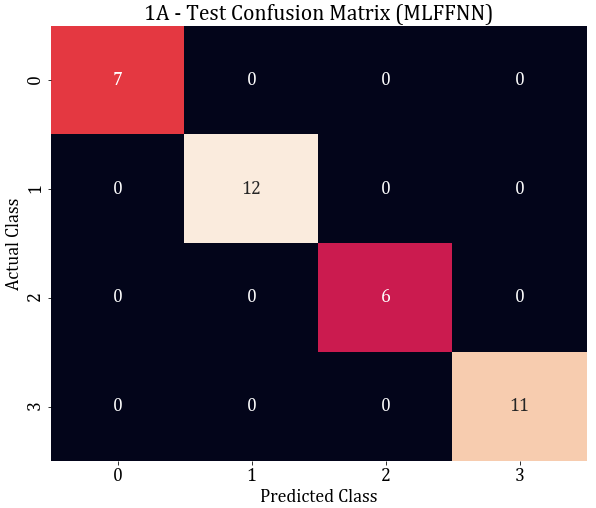
\includegraphics[scale=0.45]{images/1A_MLFFNN_test_confmat.png}
    \caption{Testing confusion matrices obtained for the best parameter combination.}
\end{figure}

\subsubsection{Decision Region}
The decision region plots obtained is as follows:
\begin{figure}[H]
    \centering
    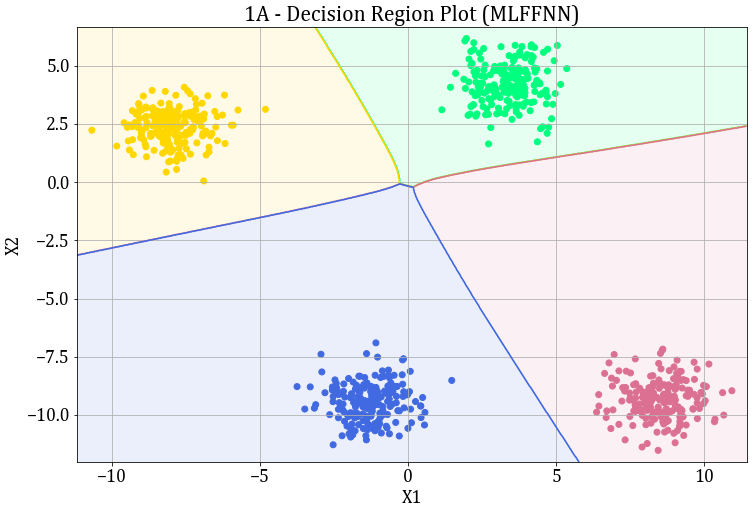
\includegraphics[scale=0.6]{images/1A_MLFFNN_Decision_Plot.png}
    \caption{Decision Region Plot obtained for the best parameter combination.}
\end{figure}

%%%%%%%%%%%%%%%%%%%%%%%%%%%%%%%%%%%%%%%%%%%%%%%
\subsection{Linear SVM}
%%%%%%%%%%%%%%%%%%%%%%%%%%%%%%%%%%%%%%%%%%%%%%%%%%

\break
%%%%%%%%%%%%%%%%%%%%%%%%%%%%%%%%%%%%%%%%%%%%%%%
%%%%%%%%%%%%%%%%%%%%%%%%%%%%%%%%%%%%%%%%%%%%%%%
\section{Dataset 1B}
This dataset contains data for three classes - 0, 1 and 2. The classes are non-linearly separable and the dimension of the feature space is 2.
%%%%%%%%%%%%%%%%%%%%%%%%%%%%%%%%%%%%%%%%%%%%%%%
%%%%%%%%%%%%%%%%%%%%%%%%%%%%%%%%%%%%%%%%%%%%%%%
\subsection{MLFFNN}
%%%%%%%%%%%%%%%%%%%%%%%%%%%%%%%%%%%%%%%%%%%%%%%%%%
The hyperparameters varied and sweeped for are - \tt{hidden layer size}, \tt{activation function}, \tt{batch size}, \tt{learning rate}, \tt{L2 regularization $\alpha$}.

\subsubsection{Classification Accuracies}
The classification accuracies on the training and validation datasets (30\% of the \colortt{dev.csv}) are as follows:
\def\arraystretch{1.25}
\begin{center}
{\small
\begin{tabular}{l l l l l l c c}
\hline
\hline
\textbf{\# Neurons} & \textbf{Activation} & \textbf{Batch Size} & \textbf{Early Stopping} & \textbf{Learning Rate} & \textbf{\alpha} & \textbf{Accuracy} & \textbf{Validation Accuracy} \\
\hline
\hline
(8, 8) & relu & 50 & False & adaptive & 0.01 & 99.33 & 98.41  \\
(8, 8) & relu & 50 & False & constant & 0.001 & 99.33 & 98.41  \\
(8, 8) & relu & 50 & False & invscaling & 0.01 & 99.33 & 98.41  \\
(8, 8) & relu & 50 & False & adaptive & 0.001 & 99.33 & 98.41  \\
(8, 8) & relu & 50 & False & invscaling & 0.001 & 99.33 & 98.41  \\
(8, 8) & relu & 50 & False & constant & 0.01 & 99.33 & 98.41  \\
(10, 10) & relu & 50 & False & adaptive & 0.01 & 99.0 & 98.41  \\
(10, 10) & relu & 50 & False & constant & 0.01 & 99.0 & 98.41  \\
(10, 10) & relu & 50 & False & invscaling & 0.01 & 99.0 & 98.41  \\
(10, 10) & relu & 50 & False & constant & 0.001 & 99.0 & 96.82  \\
\hline
\end{tabular}
\captionof{table}{Best 10 Train and Validation Accuracies obtained after performing a \colortt{GridSearch} on 432 parameter combinations.}
}
\end{center}

\subsubsection{Best Model}
The parameter combination were additionally sorted based on minimum fitting time (least fitting time - first) and the model that gave the best accuracy the fastest was chosen. Hence the best parameter combination chosen is:
\begin{itemize}
    \itemsep0em
    \item hidden\_layer\_sizes: (8, 8)
    \item activation: relu
    \item batch\_size: 50
    \item early\_stopping: False
    \item learning\_rate: adaptive
    \item alpha (L2 regularization): 0.01
\end{itemize}

\noi
The classification accuracy of the best model on the testing data is: $96.296\%$. The confusion matrices obtained are as follows:
\begin{figure}[H]
    \centering
    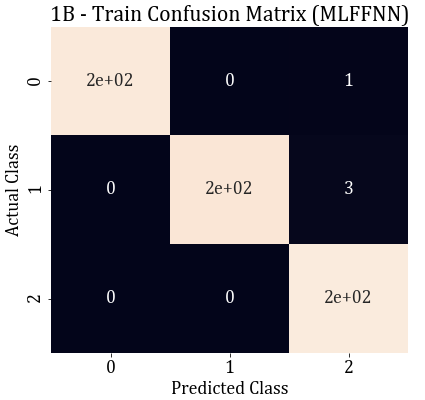
\includegraphics[scale=0.55]{images/1B_MLFFNN_train_confmat.png}
    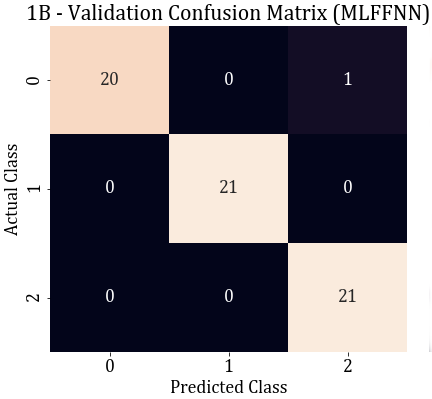
\includegraphics[scale=0.55]{images/1B_MLFFNN_val_confmat.png}
    \caption{Training and Validation confusion matrices obtained for the best parameter combination, on the left and right respectively.}
\end{figure}

\begin{figure}[H]
    \centering
    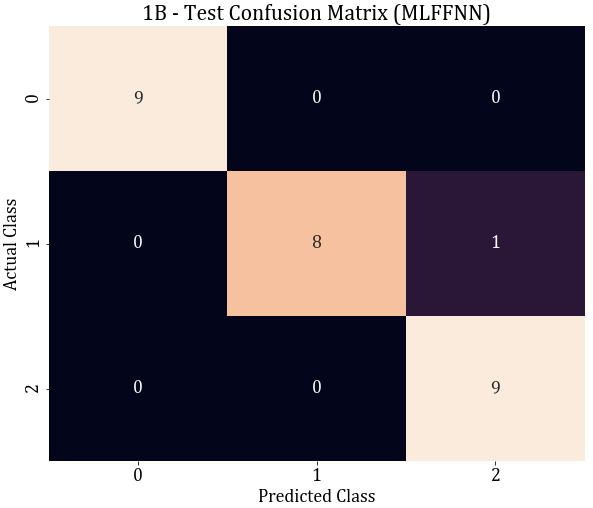
\includegraphics[scale=0.45]{images/1B_MLFFNN_test_confmat.png}
    \caption{Testing confusion matrices obtained for the best parameter combination.}
\end{figure}

\subsubsection{Decision Region}
The decision region plots obtained is as follows:
\begin{figure}[H]
    \centering
    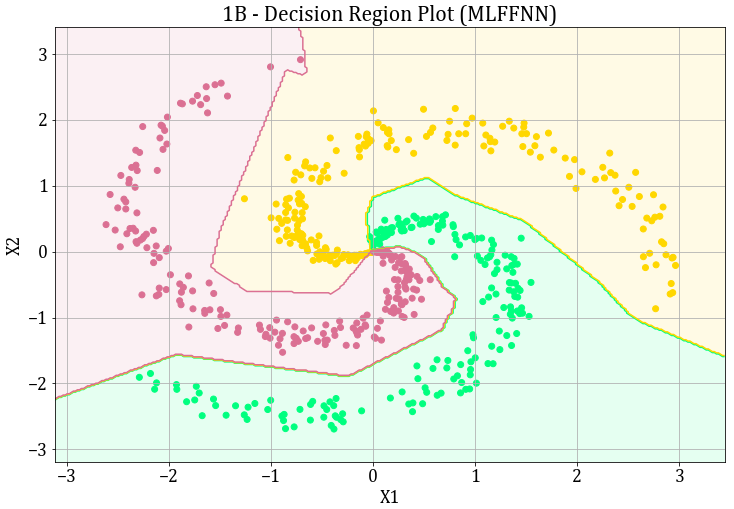
\includegraphics[scale=0.55]{images/1B_MLFFNN_Decision_Plot.png}
    \caption{Decision Region Plot obtained for the best parameter combination.}
\end{figure}

\subsubsection{Surface Plots}
The neuron-wise surface plots obtained for the hidden and output layers is as follows:
\paragraph{Hidden Layer 1, Node 1}
\begin{figure}[H]
    \centering
    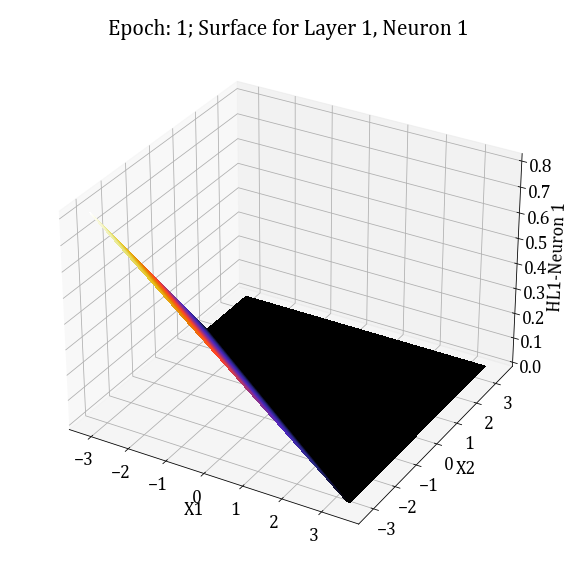
\includegraphics[scale=0.4]{images/1B_MLFFNN_E1_HL1_N1.png}
    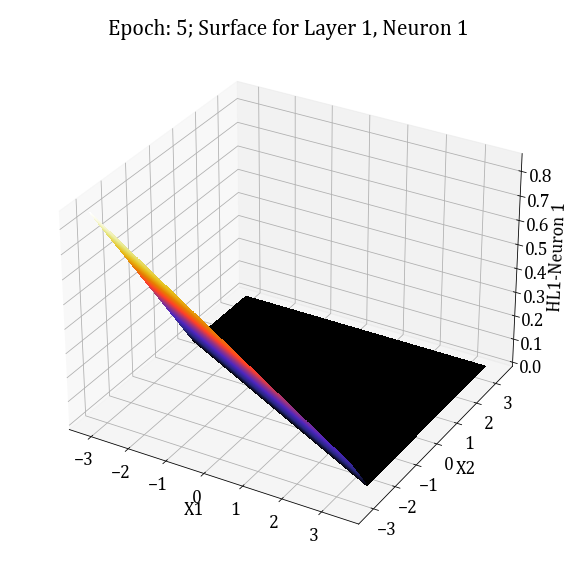
\includegraphics[scale=0.4]{images/1B_MLFFNN_E5_HL1_N1.png}
    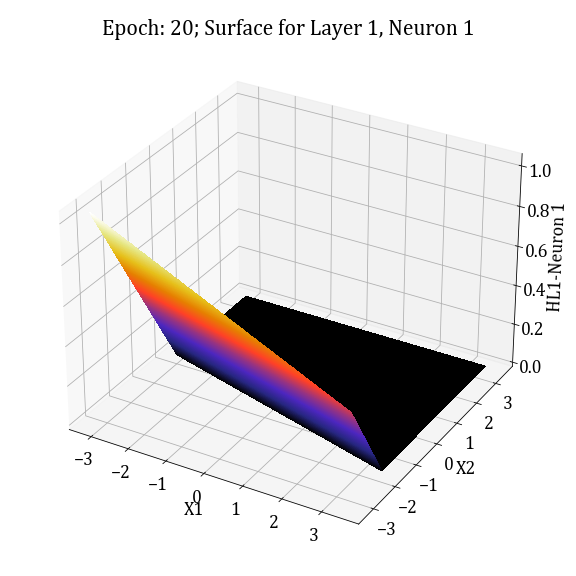
\includegraphics[scale=0.4]{images/1B_MLFFNN_E20_HL1_N1.png}
    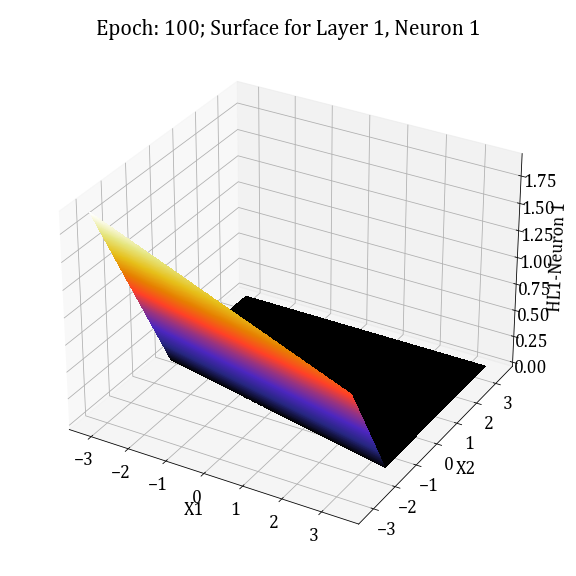
\includegraphics[scale=0.4]{images/1B_MLFFNN_E100_HL1_N1.png}
    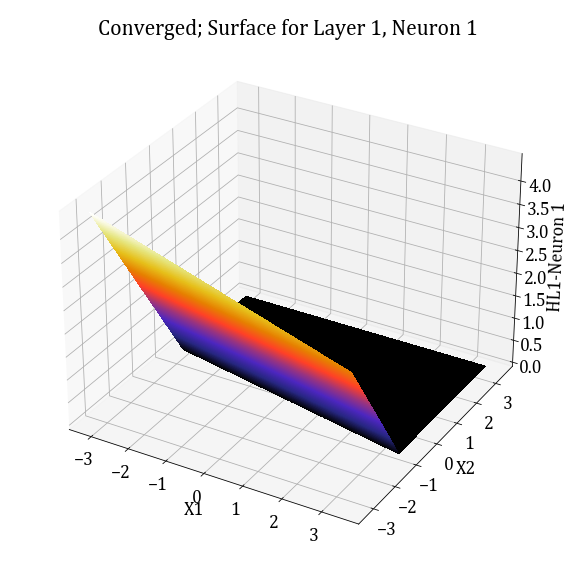
\includegraphics[scale=0.4]{images/1B_MLFFNN_conv_HL1_N1.png}
    \caption{Surface Plots obtained for Hidden Layer 1, Neuron 1, across epochs.}
    \label{HL1N1}
\end{figure}

\paragraph{Hidden Layer 1, Node 2}
\begin{figure}[H]
    \centering
    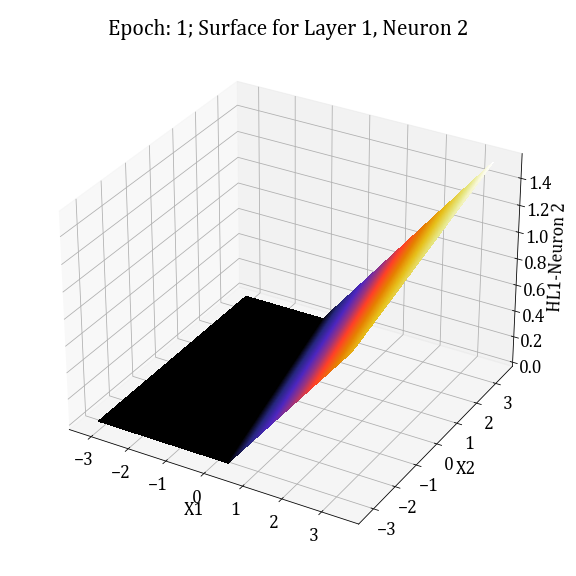
\includegraphics[scale=0.4]{images/1B_MLFFNN_E1_HL1_N2.png}
    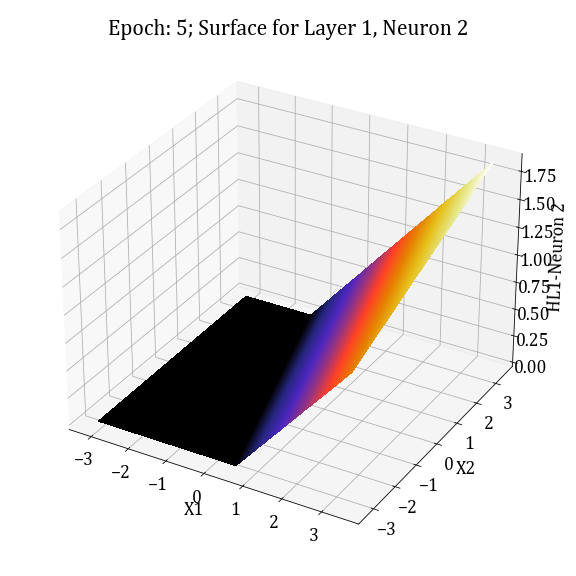
\includegraphics[scale=0.4]{images/1B_MLFFNN_E5_HL1_N2.png}
    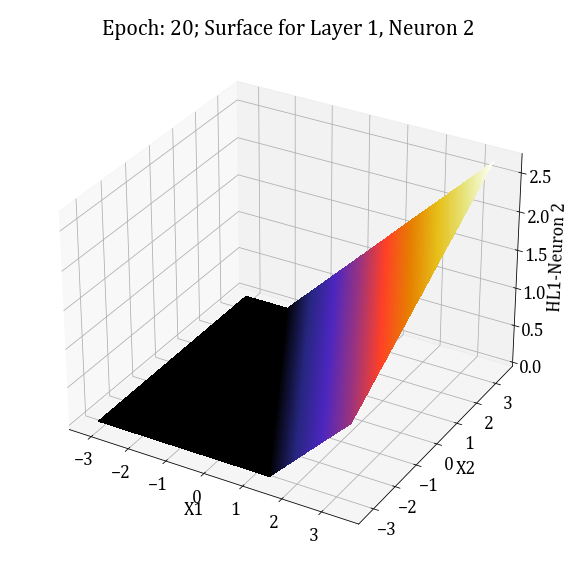
\includegraphics[scale=0.4]{images/1B_MLFFNN_E20_HL1_N2.png}
    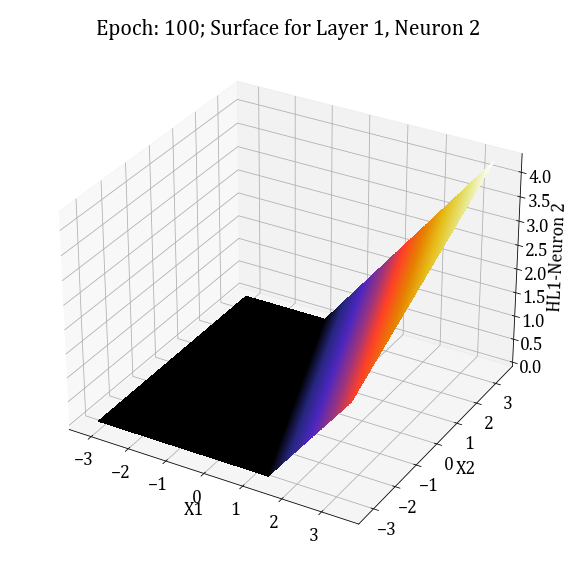
\includegraphics[scale=0.4]{images/1B_MLFFNN_E100_HL1_N2.png}
    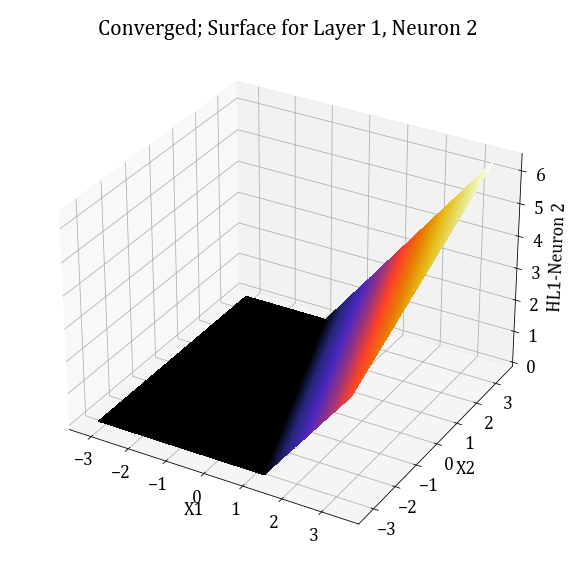
\includegraphics[scale=0.4]{images/1B_MLFFNN_conv_HL1_N2.png}
    \caption{Surface Plots obtained for Hidden Layer 1, Neuron 2, across epochs.}
\end{figure}

\paragraph{Hidden Layer 1, Node 3}
\begin{figure}[H]
    \centering
    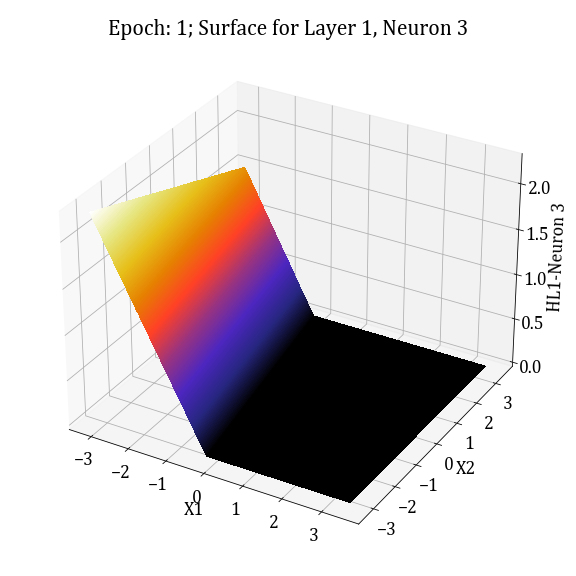
\includegraphics[scale=0.4]{images/1B_MLFFNN_E1_HL1_N3.png}
    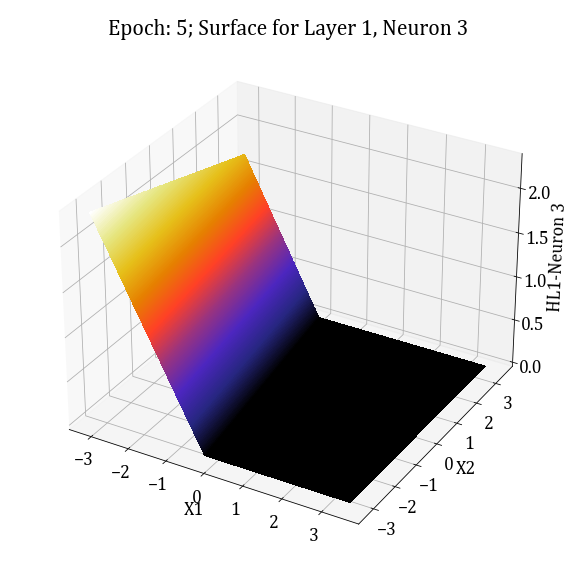
\includegraphics[scale=0.4]{images/1B_MLFFNN_E5_HL1_N3.png}
    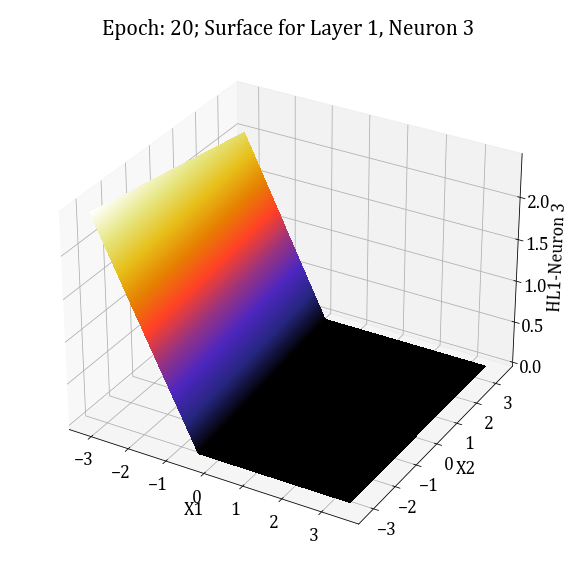
\includegraphics[scale=0.4]{images/1B_MLFFNN_E20_HL1_N3.png}
    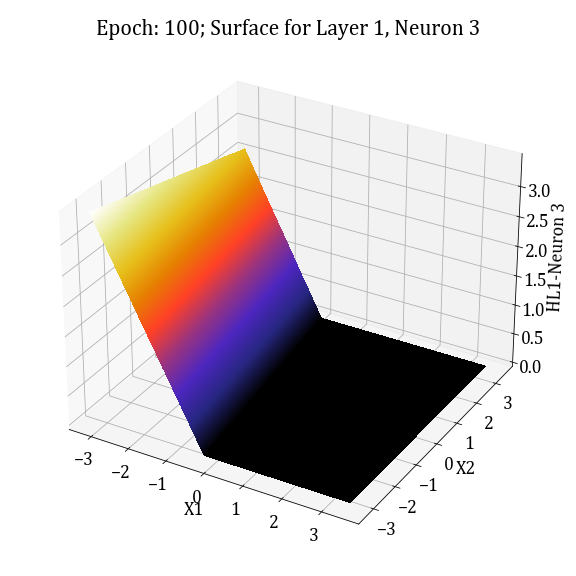
\includegraphics[scale=0.4]{images/1B_MLFFNN_E100_HL1_N3.png}
    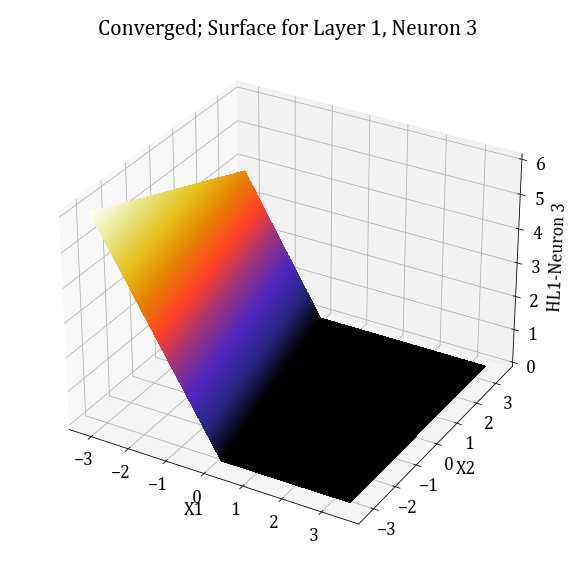
\includegraphics[scale=0.4]{images/1B_MLFFNN_conv_HL1_N3.png}
    \caption{Surface Plots obtained for Hidden Layer 1, Neuron 3, across epochs.}
\end{figure}

\paragraph{Hidden Layer 1, Node 4}
\begin{figure}[H]
    \centering
    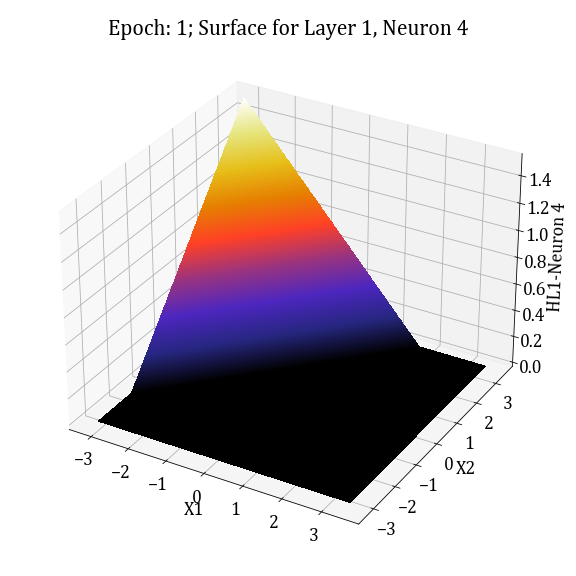
\includegraphics[scale=0.4]{images/1B_MLFFNN_E1_HL1_N4.png}
    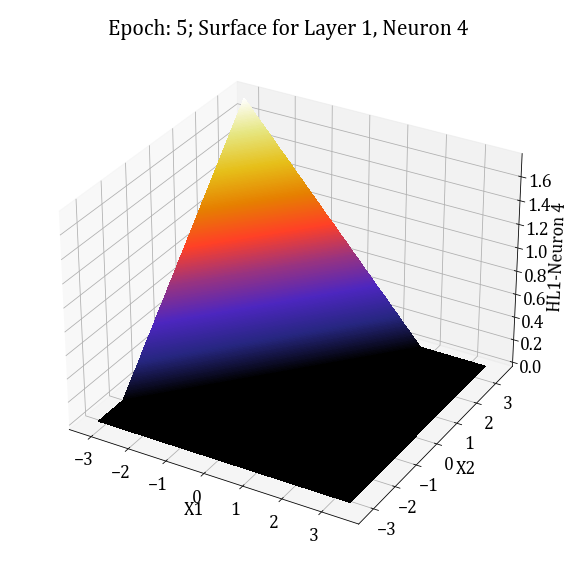
\includegraphics[scale=0.4]{images/1B_MLFFNN_E5_HL1_N4.png}
    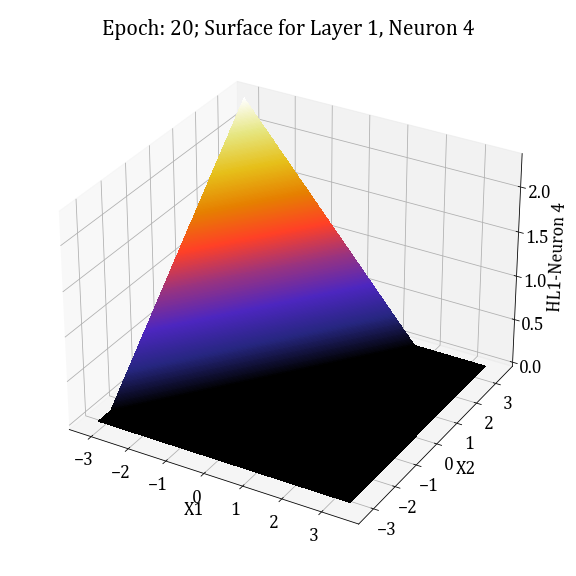
\includegraphics[scale=0.4]{images/1B_MLFFNN_E20_HL1_N4.png}
    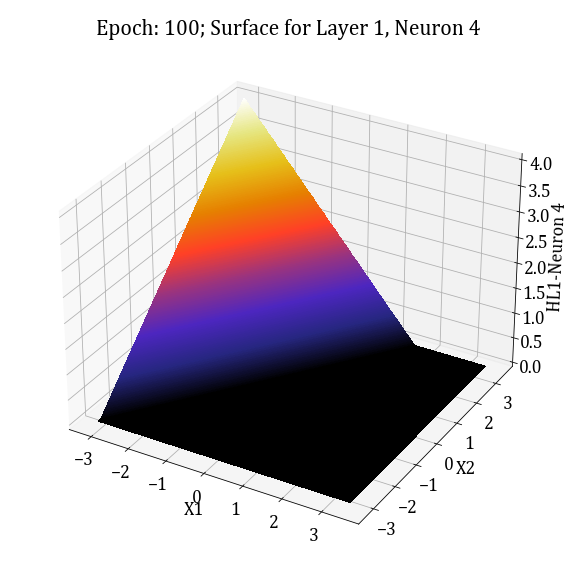
\includegraphics[scale=0.4]{images/1B_MLFFNN_E100_HL1_N4.png}
    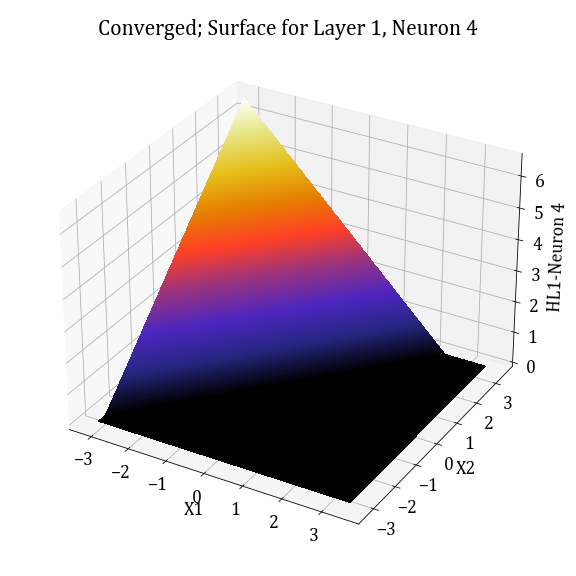
\includegraphics[scale=0.4]{images/1B_MLFFNN_conv_HL1_N4.png}
    \caption{Surface Plots obtained for Hidden Layer 1, Neuron 4, across epochs.}
\end{figure}

\paragraph{Hidden Layer 1, Node 5}
\begin{figure}[H]
    \centering
    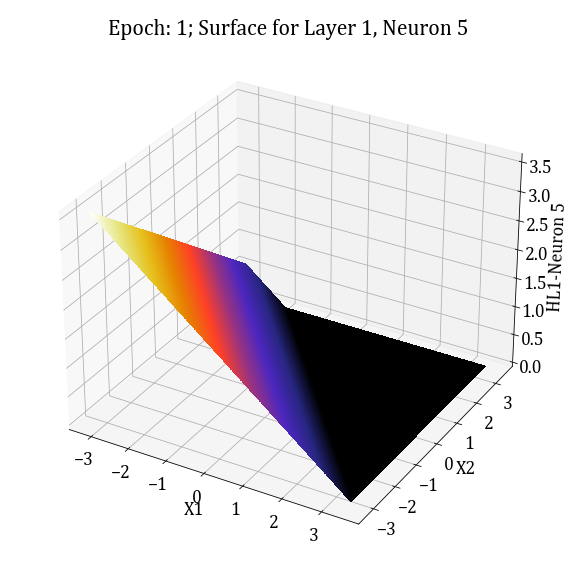
\includegraphics[scale=0.4]{images/1B_MLFFNN_E1_HL1_N5.png}
    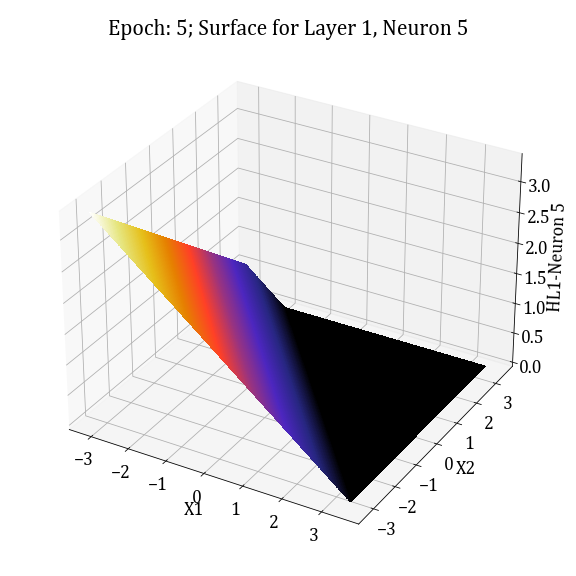
\includegraphics[scale=0.4]{images/1B_MLFFNN_E5_HL1_N5.png}
    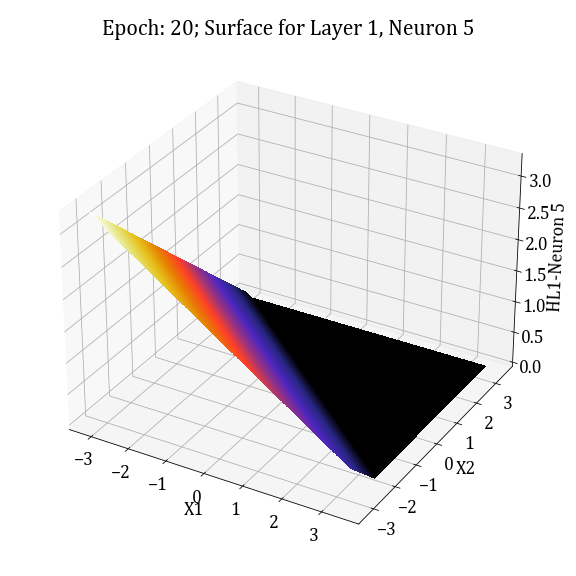
\includegraphics[scale=0.4]{images/1B_MLFFNN_E20_HL1_N5.png}
    \includegraphics[scale=0.4]{images/1B_MLFFNN_E100_HL1_N5.png}
    \includegraphics[scale=0.4]{images/1B_MLFFNN_conv_HL1_N5.png}
    \caption{Surface Plots obtained for Hidden Layer 1, Neuron 5, across epochs.}
\end{figure}

\paragraph{Hidden Layer 1, Node 6}
\begin{figure}[H]
    \centering
    \includegraphics[scale=0.4]{images/1B_MLFFNN_E1_HL1_N6.png}
    \includegraphics[scale=0.4]{images/1B_MLFFNN_E5_HL1_N6.png}
    \includegraphics[scale=0.4]{images/1B_MLFFNN_E20_HL1_N6.png}
    \includegraphics[scale=0.4]{images/1B_MLFFNN_E100_HL1_N6.png}
    \includegraphics[scale=0.4]{images/1B_MLFFNN_conv_HL1_N6.png}
    \caption{Surface Plots obtained for Hidden Layer 1, Neuron 6, across epochs.}
\end{figure}

\paragraph{Hidden Layer 1, Node 7}
\begin{figure}[H]
    \centering
    \includegraphics[scale=0.4]{images/1B_MLFFNN_E1_HL1_N7.png}
    \includegraphics[scale=0.4]{images/1B_MLFFNN_E5_HL1_N7.png}
    \includegraphics[scale=0.4]{images/1B_MLFFNN_E20_HL1_N7.png}
    \includegraphics[scale=0.4]{images/1B_MLFFNN_E100_HL1_N7.png}
    \includegraphics[scale=0.4]{images/1B_MLFFNN_conv_HL1_N7.png}
    \caption{Surface Plots obtained for Hidden Layer 1, Neuron 7, across epochs.}
\end{figure}

\paragraph{Hidden Layer 1, Node 8}
\begin{figure}[H]
    \centering
    \includegraphics[scale=0.4]{images/1B_MLFFNN_E1_HL1_N8.png}
    \includegraphics[scale=0.4]{images/1B_MLFFNN_E5_HL1_N8.png}
    \includegraphics[scale=0.4]{images/1B_MLFFNN_E20_HL1_N8.png}
    \includegraphics[scale=0.4]{images/1B_MLFFNN_E100_HL1_N8.png}
    \includegraphics[scale=0.4]{images/1B_MLFFNN_conv_HL1_N8.png}
    \caption{Surface Plots obtained for Hidden Layer 1, Neuron 8, across epochs.}
\end{figure}

\paragraph{Hidden Layer 2, Node 1}
\begin{figure}[H]
    \centering
    \includegraphics[scale=0.4]{images/1B_MLFFNN_E1_HL2_N1.png}
    \includegraphics[scale=0.4]{images/1B_MLFFNN_E5_HL2_N1.png}
    \includegraphics[scale=0.4]{images/1B_MLFFNN_E20_HL2_N1.png}
    \includegraphics[scale=0.4]{images/1B_MLFFNN_E100_HL2_N1.png}
    \includegraphics[scale=0.4]{images/1B_MLFFNN_conv_HL2_N1.png}
    \caption{Surface Plots obtained for Hidden Layer 2, Neuron 1, across epochs.}
\end{figure}

\paragraph{Hidden Layer 2, Node 2}
\begin{figure}[H]
    \centering
    \includegraphics[scale=0.4]{images/1B_MLFFNN_E1_HL2_N2.png}
    \includegraphics[scale=0.4]{images/1B_MLFFNN_E5_HL2_N2.png}
    \includegraphics[scale=0.4]{images/1B_MLFFNN_E20_HL2_N2.png}
    \includegraphics[scale=0.4]{images/1B_MLFFNN_E100_HL2_N2.png}
    \includegraphics[scale=0.4]{images/1B_MLFFNN_conv_HL2_N2.png}
    \caption{Surface Plots obtained for Hidden Layer 2, Neuron 2, across epochs.}
\end{figure}

\paragraph{Hidden Layer 2, Node 3}
\begin{figure}[H]
    \centering
    \includegraphics[scale=0.4]{images/1B_MLFFNN_E1_HL2_N3.png}
    \includegraphics[scale=0.4]{images/1B_MLFFNN_E5_HL2_N3.png}
    \includegraphics[scale=0.4]{images/1B_MLFFNN_E20_HL2_N3.png}
    \includegraphics[scale=0.4]{images/1B_MLFFNN_E100_HL2_N3.png}
    \includegraphics[scale=0.4]{images/1B_MLFFNN_conv_HL2_N3.png}
    \caption{Surface Plots obtained for Hidden Layer 2, Neuron 3, across epochs.}
\end{figure}

\paragraph{Hidden Layer 2, Node 4}
\begin{figure}[H]
    \centering
    \includegraphics[scale=0.4]{images/1B_MLFFNN_E1_HL2_N4.png}
    \includegraphics[scale=0.4]{images/1B_MLFFNN_E5_HL2_N4.png}
    \includegraphics[scale=0.4]{images/1B_MLFFNN_E20_HL2_N4.png}
    \includegraphics[scale=0.4]{images/1B_MLFFNN_E100_HL2_N4.png}
    \includegraphics[scale=0.4]{images/1B_MLFFNN_conv_HL2_N4.png}
    \caption{Surface Plots obtained for Hidden Layer 2, Neuron 4, across epochs.}
\end{figure}

\paragraph{Hidden Layer 2, Node 5}
\begin{figure}[H]
    \centering
    \includegraphics[scale=0.4]{images/1B_MLFFNN_E1_HL2_N5.png}
    \includegraphics[scale=0.4]{images/1B_MLFFNN_E5_HL2_N5.png}
    \includegraphics[scale=0.4]{images/1B_MLFFNN_E20_HL2_N5.png}
    \includegraphics[scale=0.4]{images/1B_MLFFNN_E100_HL2_N5.png}
    \includegraphics[scale=0.4]{images/1B_MLFFNN_conv_HL2_N5.png}
    \caption{Surface Plots obtained for Hidden Layer 2, Neuron 5, across epochs.}
\end{figure}

\paragraph{Hidden Layer 2, Node 6}
\begin{figure}[H]
    \centering
    \includegraphics[scale=0.4]{images/1B_MLFFNN_E1_HL2_N6.png}
    \includegraphics[scale=0.4]{images/1B_MLFFNN_E5_HL2_N6.png}
    \includegraphics[scale=0.4]{images/1B_MLFFNN_E20_HL2_N6.png}
    \includegraphics[scale=0.4]{images/1B_MLFFNN_E100_HL2_N6.png}
    \includegraphics[scale=0.4]{images/1B_MLFFNN_conv_HL2_N6.png}
    \caption{Surface Plots obtained for Hidden Layer 2, Neuron 6, across epochs.}
\end{figure}

\paragraph{Hidden Layer 2, Node 7}
\begin{figure}[H]
    \centering
    \includegraphics[scale=0.4]{images/1B_MLFFNN_E1_HL2_N7.png}
    \includegraphics[scale=0.4]{images/1B_MLFFNN_E5_HL2_N7.png}
    \includegraphics[scale=0.4]{images/1B_MLFFNN_E20_HL2_N7.png}
    \includegraphics[scale=0.4]{images/1B_MLFFNN_E100_HL2_N7.png}
    \includegraphics[scale=0.4]{images/1B_MLFFNN_conv_HL2_N7.png}
    \caption{Surface Plots obtained for Hidden Layer 2, Neuron 7, across epochs.}
\end{figure}

\paragraph{Hidden Layer 2, Node 8}
\begin{figure}[H]
    \centering
    \includegraphics[scale=0.4]{images/1B_MLFFNN_E1_HL2_N8.png}
    \includegraphics[scale=0.4]{images/1B_MLFFNN_E5_HL2_N8.png}
    \includegraphics[scale=0.4]{images/1B_MLFFNN_E20_HL2_N8.png}
    \includegraphics[scale=0.4]{images/1B_MLFFNN_E100_HL2_N8.png}
    \includegraphics[scale=0.4]{images/1B_MLFFNN_conv_HL2_N8.png}
    \caption{Surface Plots obtained for Hidden Layer 2, Neuron 8, across epochs.}
\end{figure}

\paragraph{Output Layer, Node 1}
\begin{figure}[H]
    \centering
    \includegraphics[scale=0.4]{images/1B_MLFFNN_E1_OP_N1.png}
    \includegraphics[scale=0.4]{images/1B_MLFFNN_E5_OP_N1.png}
    \includegraphics[scale=0.4]{images/1B_MLFFNN_E20_OP_N1.png}
    \includegraphics[scale=0.4]{images/1B_MLFFNN_E100_OP_N1.png}
    \includegraphics[scale=0.4]{images/1B_MLFFNN_conv_OP_N1.png}
    \caption{Surface Plots obtained for Output Layer, Neuron 1, across epochs.}
\end{figure}

\paragraph{Output Layer, Node 2}
\begin{figure}[H]
    \centering
    \includegraphics[scale=0.4]{images/1B_MLFFNN_E1_OP_N2.png}
    \includegraphics[scale=0.4]{images/1B_MLFFNN_E5_OP_N2.png}
    \includegraphics[scale=0.4]{images/1B_MLFFNN_E20_OP_N2.png}
    \includegraphics[scale=0.4]{images/1B_MLFFNN_E100_OP_N2.png}
    \includegraphics[scale=0.4]{images/1B_MLFFNN_conv_OP_N2.png}
    \caption{Surface Plots obtained for Output Layer, Neuron 2, across epochs.}
\end{figure}

\paragraph{Output Layer, Node 3}
\begin{figure}[H]
    \centering
    \includegraphics[scale=0.4]{images/1B_MLFFNN_E1_OP_N3.png}
    \includegraphics[scale=0.4]{images/1B_MLFFNN_E5_OP_N3.png}
    \includegraphics[scale=0.4]{images/1B_MLFFNN_E20_OP_N3.png}
    \includegraphics[scale=0.4]{images/1B_MLFFNN_E100_OP_N3.png}
    \includegraphics[scale=0.4]{images/1B_MLFFNN_conv_OP_N3.png}
    \caption{Surface Plots obtained for Output Layer, Neuron 3, across epochs.}
    \label{OPN3}
\end{figure}

\noi
From \autoref{HL1N1}-\autoref{OPN3}, we observe the following:
\begin{itemize}
    \itemsep0em 
    \item First hidden layer surface plot is non-linear (activation function is \colortt{ReLU}). However, the surfaces obtained are hyperplanes.
    \item Responses from the second layer is highly non-linear and the surfaces are very comples.
    \item The surface plot of the output neurons shows the selection cum localization of different classes in the latent space.
\end{itemize}

%%%%%%%%%%%%%%%%%%%%%%%%%%%%%%%%%%%%%%%%%%%%%%%
\subsection{Non-Linear SVM}

%%%%%%%%%%%%%%%%%%%%%%%%%%%%%%%%%%%%%%%%%%%%%%%
\break
%%%%%%%%%%%%%%%%%%%%%%%%%%%%%%%%%%%%%%%%%%%%%%%
\section{Dataset 2A}
%%%%%%%%%%%%%%%%%%%%%%%%%%%%%%%%%%%%%%%%%%%%%%%
%%%%%%%%%%%%%%%%%%%%%%%%%%%%%%%%%%%%%%%%%%%%%%%
This dataset contains data for five classes. The classes assigned for our team are: \tt{coast}, \tt{highway}, \tt{mountain}, \tt{opencountry} and \tt{tallbuilding}. These classes were assigned the class label 0, 1, 2, 3 and 4 respectively. The classes are non-linearly separable and the dimension of the feature space is 24.

%%%%%%%%%%%%%%%%%%%%%%%%%%%%%%%%%%%%%%%%%%%%%%%
\subsection{MLFFNN}
%%%%%%%%%%%%%%%%%%%%%%%%%%%%%%%%%%%%%%%%%%%%%%%
An initial parameter search by varying the parameters of the MLFFNN alone was done. However, the accuracy of the model couldn't be improved. In order to increase the accuracy of the model, PCA was used to reduce the dimensionality of the model.\\

\noi
The hyperparameters varied and sweeped for are - \tt{PCA \# components} \tt{MLFFNN hidden layer size}, \tt{MLFFNN batch size}, \tt{MLFFNN learning rate} and \tt{MLFFNN L2 regularization $\alpha$}.

\subsubsection{Classification Accuracies}
The classification accuracies on the training and validation datasets (30\% of the \colortt{dev.csv}) are as follows:
\def\arraystretch{1.25}
\begin{center}
{\small
\begin{tabular}{l l l l l l c c}
\hline
\hline
\textbf{\# Components} & \textbf{\# Neurons} & \textbf{Learning Rate} & \textbf{Batch Size} & \textbf{\alpha} & \textbf{Accuracy} & \textbf{Validation Accuracy} \\
\hline
\hline
16 & (50, 50) & invscaling & auto & 0.001 & 79.02 & 52.23 \\
16 & (50, 50) & adaptive & auto & 0.001 & 79.02 & 52.23 \\
16 & (50, 50) & constant & auto & 0.001 & 79.02 & 52.23 \\
20 & (50, 50) & constant & auto & 0.010 & 82.93 & 51.82 \\
20 & (50, 50) & adaptive & auto & 0.010 & 82.93 & 51.82 \\
20 & (50, 50) & invscaling & auto & 0.010 & 82.93 & 51.82 \\
8 & (75, 75) & invscaling & 100 & 0.010 & 75.45 & 51.82 \\
19 & (25, 25) & adaptive & auto & 0.001 & 68.05 & 51.42 \\
19 & (25, 25) & constant & auto & 0.001 & 68.05 & 51.42 \\
19 & (25, 25) & invscaling & auto & 0.001 & 68.05 & 51.42 \\
\hline
\end{tabular}
\captionof{table}{Best 10 Train and Validation Accuracies obtained after performing a \colortt{GridSearch} on 1728 parameter combinations.}
}
\end{center}

\subsubsection{Best Model}
The parameter combination were additionally sorted based on minimum fitting time (least fitting time - first) and the model that gave the best accuracy the fastest (and potentially the most minimal model that best fits the data), was chosen. Hence the best parameter combination chosen is:
\begin{itemize}
    \itemsep0em
    \item n\_components: 16
    \item hidden\_layer\_sizes: (50, 50)
    \item batch\_size: 200
    \item alpha: 0.001
    \item learning\_rate: invscaling
\end{itemize}

\noi
The classification accuracy of the best model on the testing data is: $49.06\%$. \\

\noi
The confusion matrices obtained are as follows:
\begin{figure}[H]
    \centering
    \includegraphics[scale=0.4]{images/2A_MLFFNN_train_confmat.png}
    \includegraphics[scale=0.4]{images/2A_MLFFNN_val_confmat.png}
    \caption{Training and Validation confusion matrices obtained for the best parameter combination, on the left and right respectively.}
\end{figure}

\begin{figure}[H]
    \centering
    \includegraphics[scale=0.45]{images/2A_MLFFNN_test_confmat.png}
    \caption{Testing confusion matrices obtained for the best parameter combination.}
\end{figure}


\subsection{Gaussian-kernel SVM}

\end{document}
